\section{Ligand Field Assembly}

\subsection{Subsets of octahedral space}
The full combinatorial space of all ligands generated in Section \ref{sec:enum} is vast with a lower estimated bound of $> 1.8 \cdot 10^{14}$, calculated from cube coloring theorem. The difficulty is to include bidentate symmetry into the calculations. In the following, we will motivate why only a fraction of the full space is of interest. This will give us the possibility of actually enumerating the ligand fields and calculate properties of the subsets.
One goal of this work is to be able to fine tune molecular properties such as oxidation energy or spin splitting energy. It seems natural to assume that a full set of all possible ligand fields gives the most fine grained raster over all possible properties, a complex could have. This might be statistically true but also prevent rigorous analysis. The set is too dense to traverse on a computationally feasible time scale. We propose the homoleptic subset of the octahedral space as a backbone. Conceptually, homoleptic octahedral compounds must be on the edge of the actual octahedral space, since the properties of single complexes do not get more distinct than in homoleptic ones. From the homoleptic complex space it is possible to go to lower symmetry classes and get closer to a complex with desired properties without analyzing all complexes on the way. This reduces computational cost by several orders of magnitude. Our selection of complexes can be found in Table \ref{tab:space-sizes}. They were chosen to be of highest possible symmetry to result in the smallest number of complexes and to be synthetically interesting. 
\begin{table}[]
	\centering
	\caption{The sizes of the selected subsets of octahedral space.}
	\label{tab:space-sizes}
	\begin{tabular}{llr}
		\toprule
		Set 					& description		    	   & size \\
		\midrule
		Homoleptics             & eq = ax                   & 553        \\[0.1cm]
		"5+1" symmetric         & eq = ax1 $\neq$ ax2       & 163,620    \\[0.1cm]
		"4+2" symmetric         & eq1 $\neq$ eq2 = ax       & 185,376    \\[0.1cm]
		Strongly symmetric      & eq $\neq$ ax              & 245,316    \\[0.1cm]
		Equatorially asymmetric & eq1 $\neq$ eq2 $\neq$ ax  & 15,924,796 \\[0.1cm]
		Weakly symmetric        & eq $\neq$ ax1 $\neq$ ax2  & 45,077,310 \\[0.1cm]
		Complete Heteroleptics  & $L_i \neq L_j$            & $\approx 5.9 \cdot 10^{12}$ \\[0.1cm] %405!/399!/6!+148!/145!/3!
		Octahedral Space        & all                       & $> 1.8 \cdot 10^{14}$ \\
		%number of cube colorings as lower bound
		\bottomrule
	\end{tabular}
\end{table}




%\subsection{Properties of the sets}
%\begin{itemize}
%\item Reduce space to facilitate sampling from non-homoleptics
%\item Example: strongly symmetric, monodentate ligand fields (163,620)
%\item Exclude all with charge smaller than -4, which results in 87,150 ligand fields (53~\%).
%\end{itemize}
%\begin{figure}[ht] 
%	\begin{minipage}[b]{0.5\linewidth}
%		\centering
%		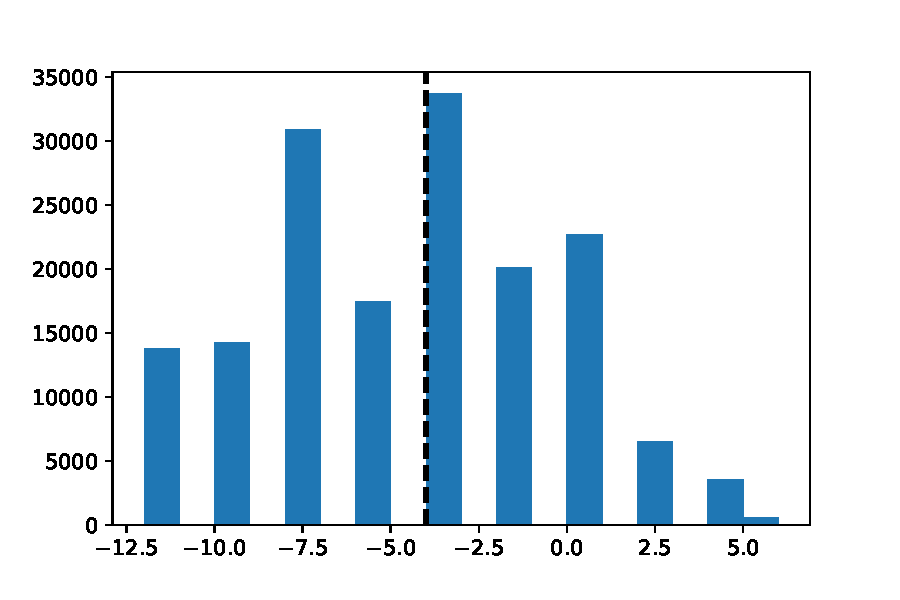
\includegraphics[width=.8\linewidth]{img/strongsymMonodentates_chargeHist.pdf} 
%		\vspace{4ex}
%	\end{minipage}%%
%	\begin{minipage}[b]{0.5\linewidth}
%		\centering
%		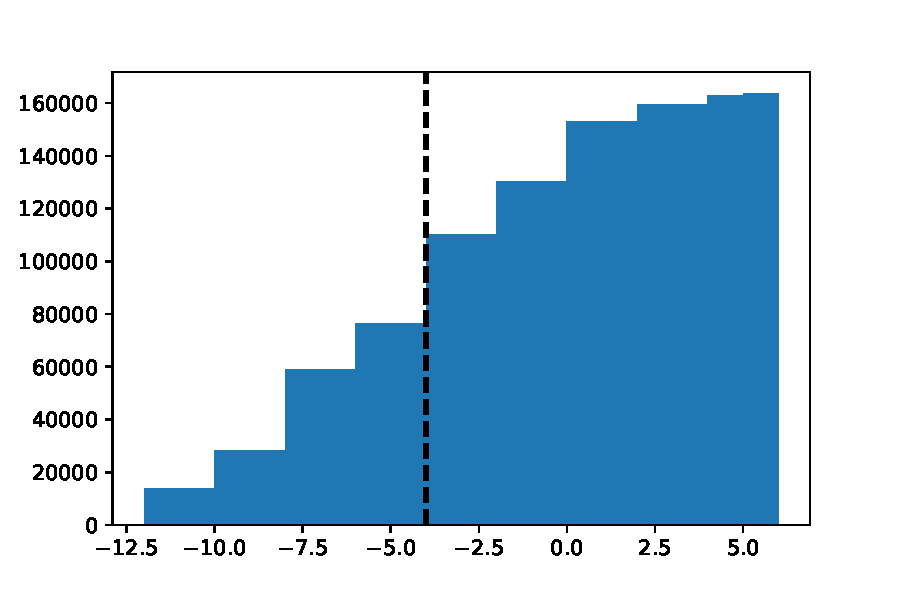
\includegraphics[width=.8\linewidth]{img/strongsymMonodentates_chargeHistCum.pdf} 
%		\vspace{4ex}
%	\end{minipage} 
%\end{figure}

\subsection{Subset analysis}
We did a principal component analysis on the homoleptic subspace and projected the strongly symmetric and "5+1" symmetric subspace onto it (see Figure \ref{fig:pca}). The connecting atom is colored according to the CPK coloring with a gradient transition from oxygen (red) to phosphorus(orange). The connecting atom is the average over all 6 connecting atoms. We can see that the gap on PC2 separates first period elements from second order elements in the homoleptic case. Going to lower symmetry, we see that this gap is filled up with fractional element types. This sonsolidates our hypothesis that the homoleptics build the backbone of the full space and that lowering symmetry allows us to find more fine grained complexes.

\begin{figure}
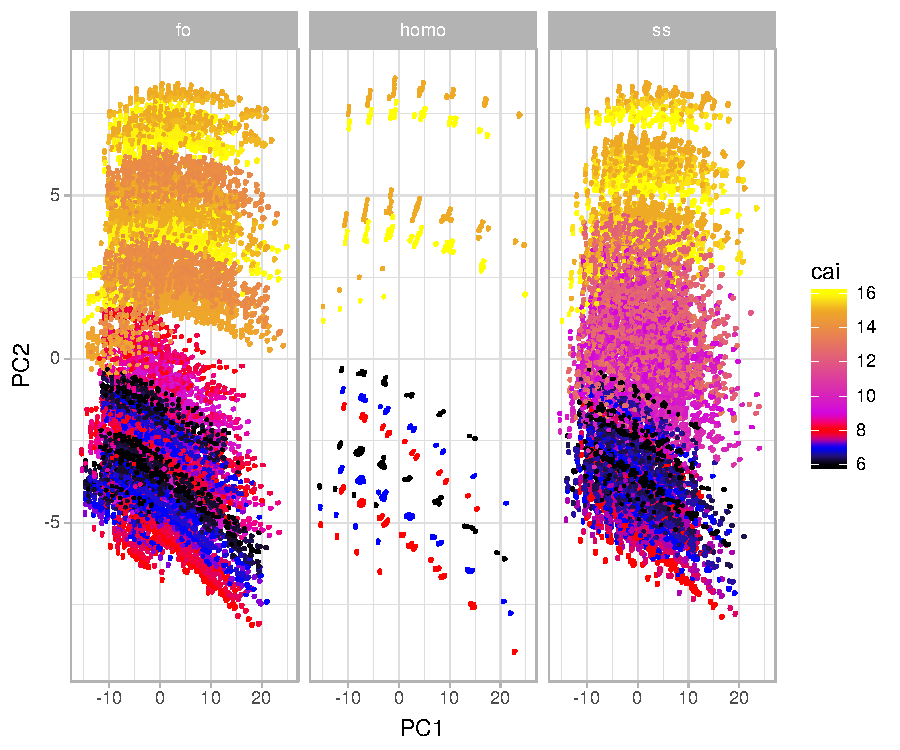
\includegraphics[width=0.7\linewidth]{img/pca.pdf}
\centering
\caption{A PCA on the homoleptic subspace. The strongly symmetric (ss) and "5+1" symmetric (fo) subspace were projected onto it. The connecting atom identity (cai) is encoded in the color following CPK coloring with a gradient transition from oxygen (red) to phosphorus (orange).}
\label{fig:pca} 
\end{figure}

\subsection{Entropy of the subsets}
To compare the different subsets, we devised a non-unqiue footprint to characterize the ligand fields in 5 dimensions:
\begin{itemize}
\item total charge
\item total valence electrons
\item electronegativity of the connecting atom
\item $^{\textrm{lc}}_{\textrm{ax,eq}}\chi_1 = \sum{EN_{\textrm{CA}} \cdot EN_i}$
\item $^{\textrm{lc}}_{\textrm{ax,eq}}\chi^\prime_1 = \sum{EN_{\textrm{CA}} - EN_i}$
\end{itemize}

We then calculate the entropy, $H_{\textrm{KDE}}$, of the Kernel Density Estimated (KDE) distrbution and Scott's rule to estimate the bandwidth of the KDE:





%\frametitle{Correlation analysis for strongly symmetric monodentates }
%\begin{figure}
%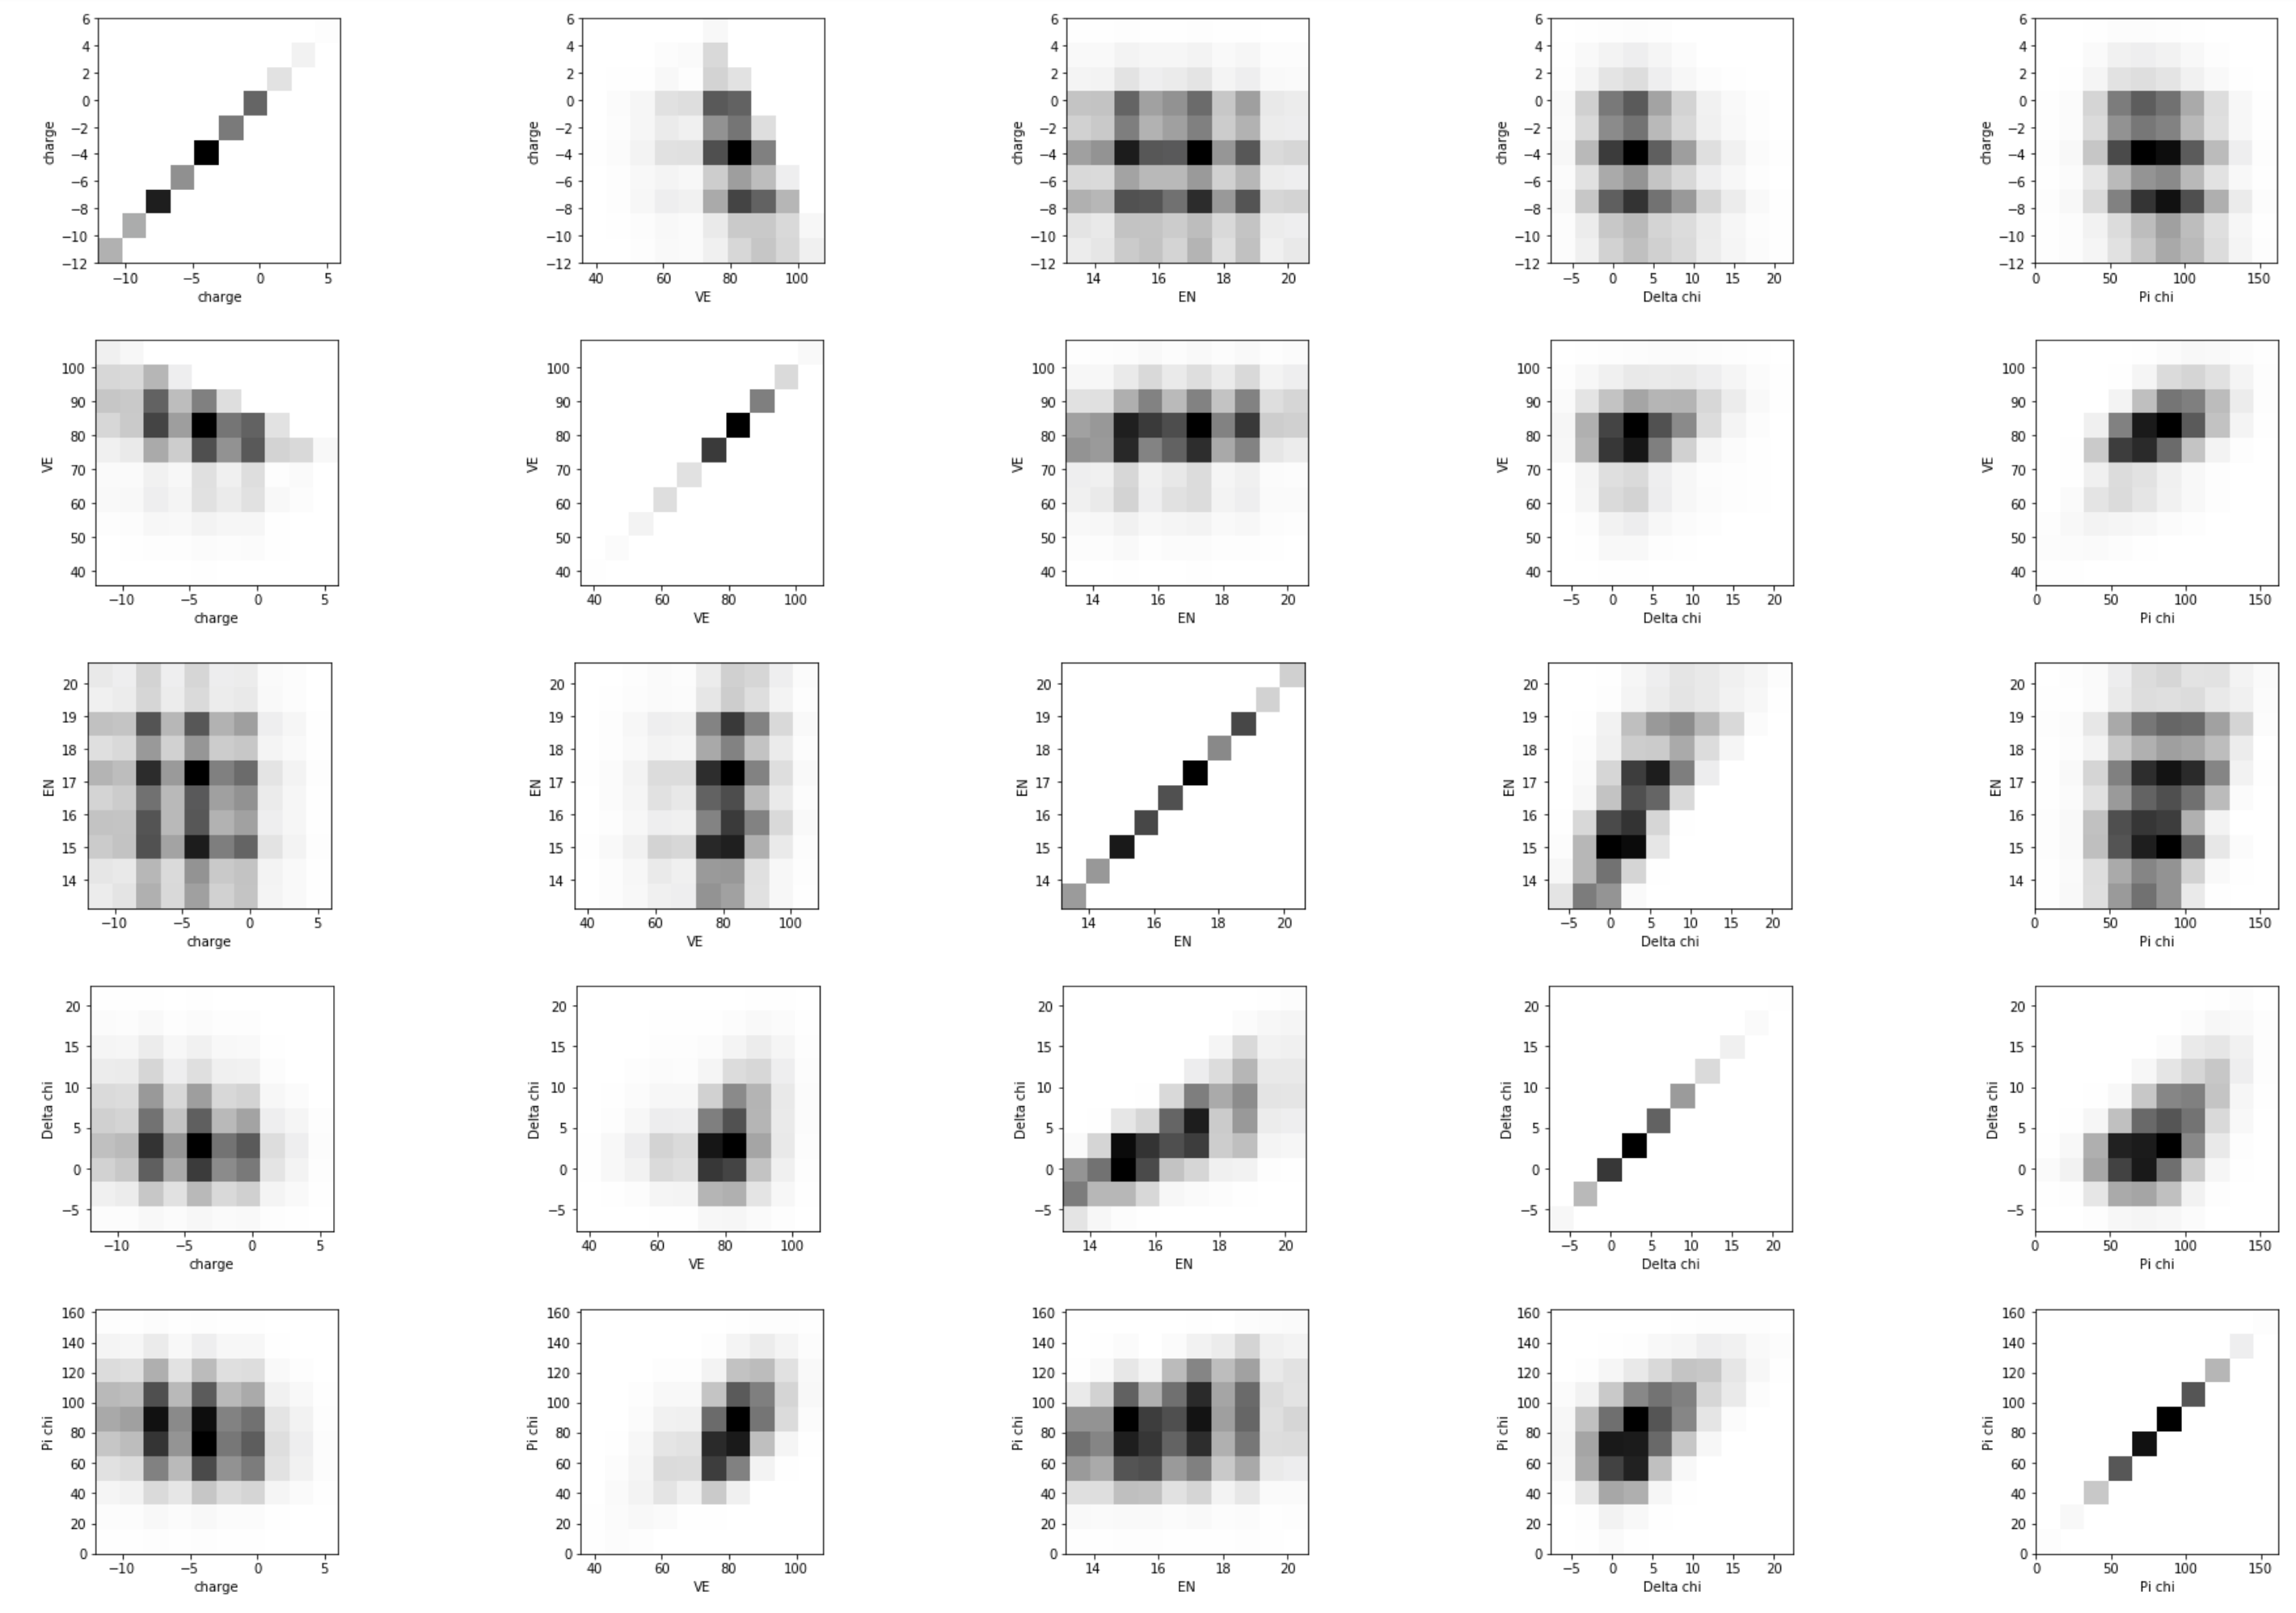
\includegraphics[width=0.65\linewidth]{img/strongsymMonodentates_PairwiseCorr.png}
%\end{figure}
%\end{frame}
%
%\begin{frame}
%\frametitle{Example of KDE slice}
%Dimensions $^{\textrm{lc}}_{\textrm{ax,eq}}\chi_1$ vs. charge in $H_{\textrm{KDE}}$ for strongly symmetric monodentates.
%\begin{figure}[ht] 
%	\begin{minipage}[b]{0.5\linewidth}
%		\centering
%		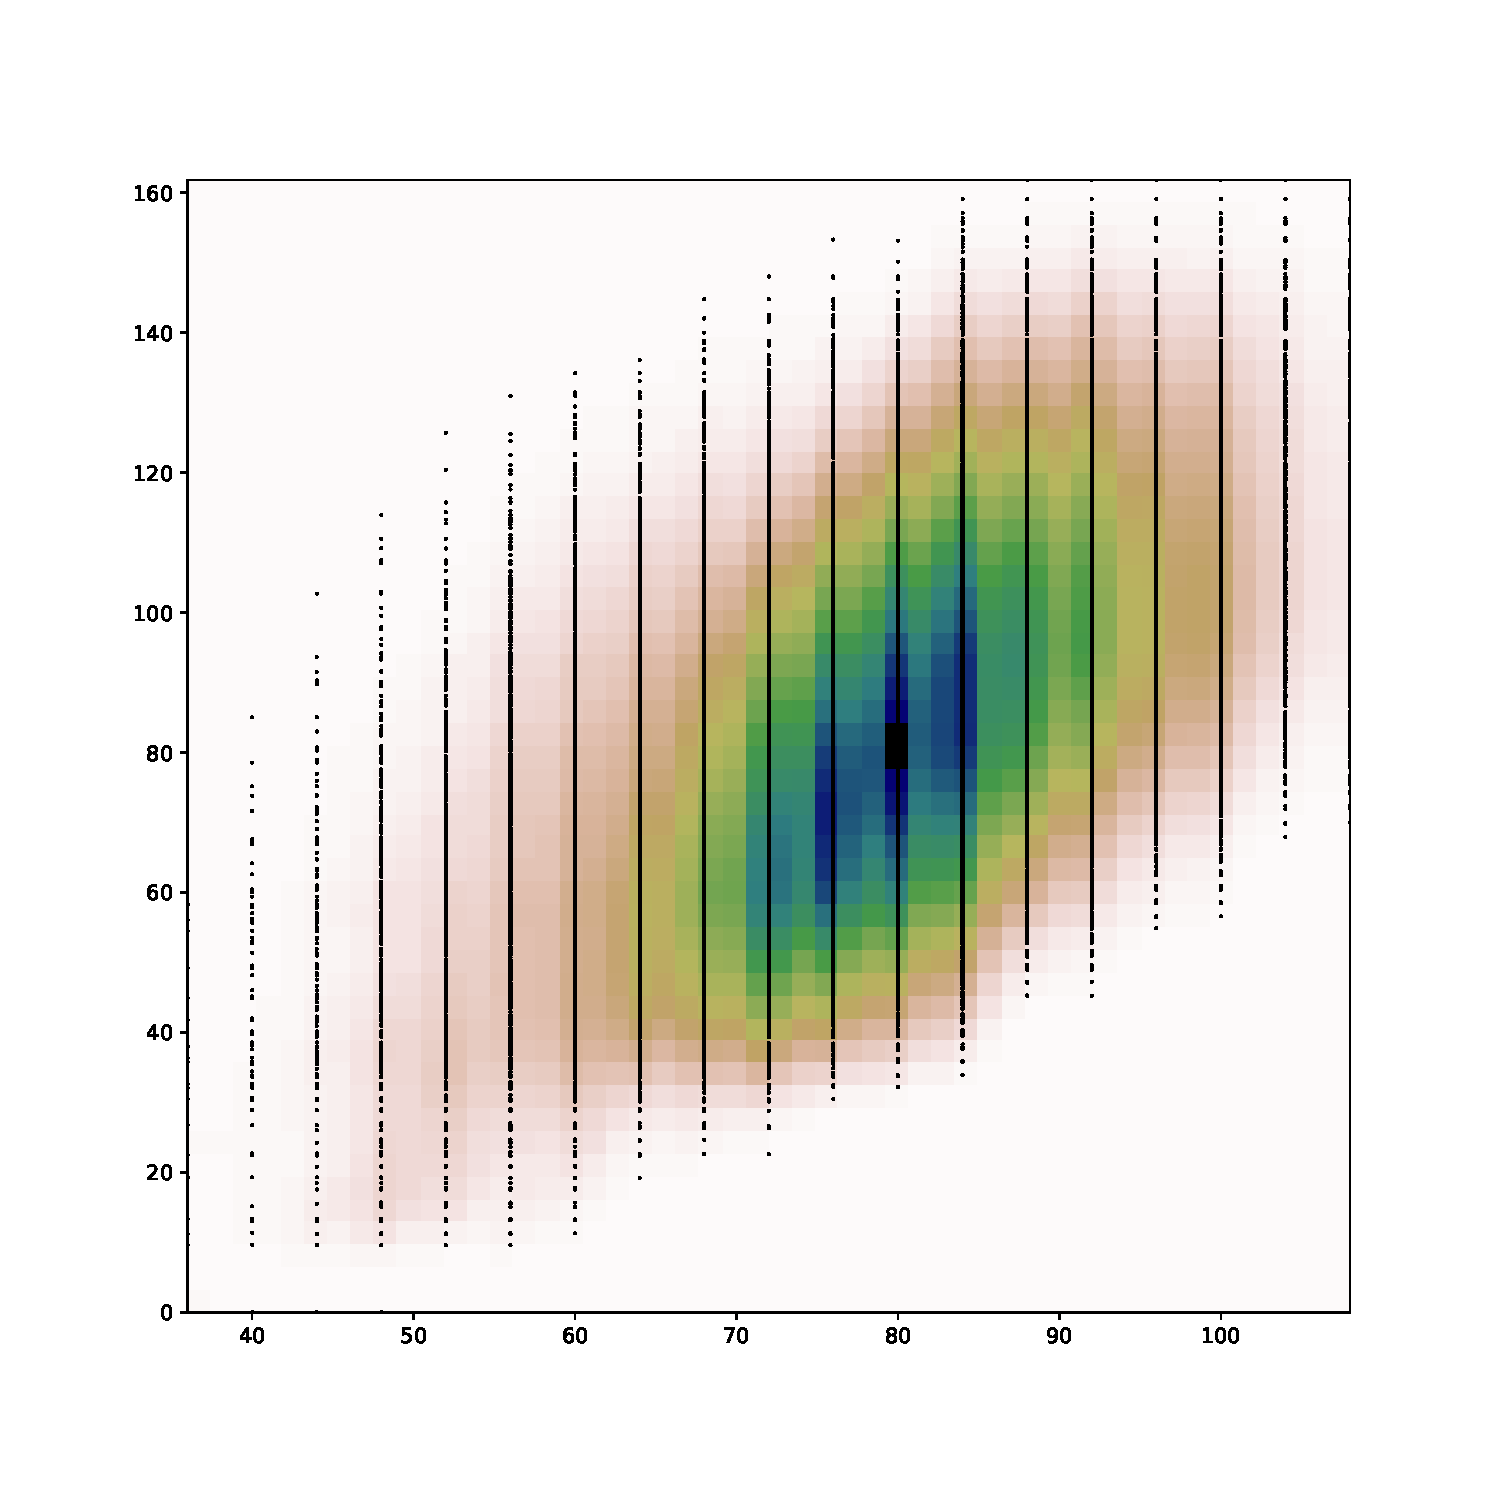
\includegraphics[width=1\linewidth]{img/strongsymMonodentates_heatmap.pdf} 
%		\vspace{2ex}
%	\end{minipage}%%
%	\begin{minipage}[b]{0.5\linewidth}
%		\centering
%		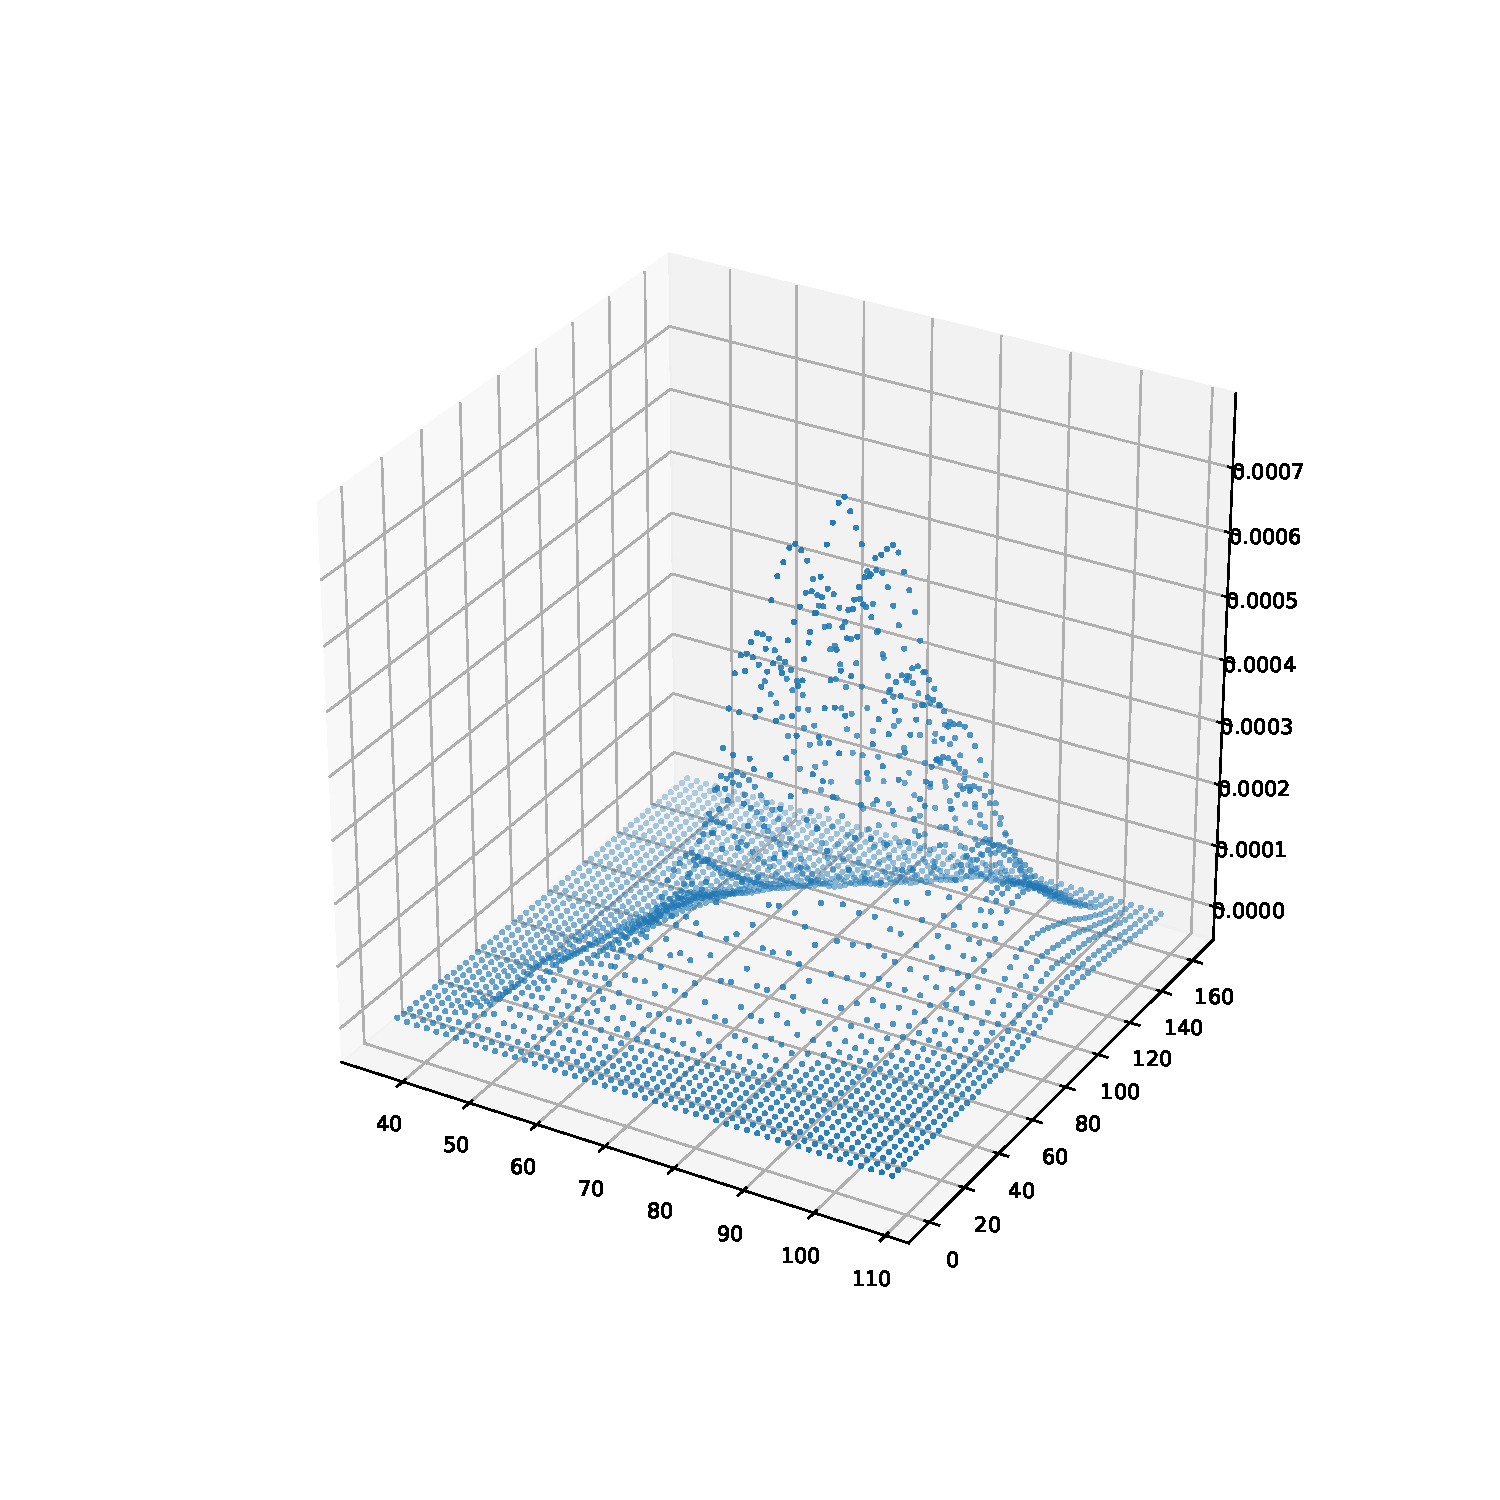
\includegraphics[width=1\linewidth]{img/strongsymMonodentates_3Dhists.pdf} 
%		\vspace{2ex}
%	\end{minipage} 
%\end{figure}
%\end{frame}
%
%\begin{frame}
%\frametitle{Monodentate Footprints}
%	\begin{table}[]
%	\centering
%	\caption{Entropic footprint}
%	\label{tab:ent-footprint}
%	\begin{tabular}{lcr}
%		\toprule
%		Set 					    &  $H_{\textrm{KDE}}^{\textrm{monodent}}$   & $H_{\textrm{KDE}}^{\textrm{bident}}$ \\
%		\midrule
%		Homoleptics                 &  19.7  & 15.63   \\[0.1cm]
%		"5+1" symmetric             &  13.7  & -       \\[0.1cm]
%		Strongly symmetric AC       &  -     & 9.47    \\[0.1cm]
%		Strongly symmetric ADC      &  12.70 & 5.53    \\[0.1cm]
%		"4+2" symmetric             &  12.70 & 9.47    \\[0.1cm] 
%		Weakly symmetric            &  8.1   & 7.7     \\[0.1cm]
%		Equatorially asymmetric AC  &  -     & 10.04   \\[0.1cm]
%		Equatorially asymmetric ADC &        &         \\[0.1cm]
%
%		\bottomrule
%	\end{tabular}
%	\end{table}
%\end{frame}
%
%\begin{frame}
%\frametitle{Entropy histogram}
%\begin{figure}
%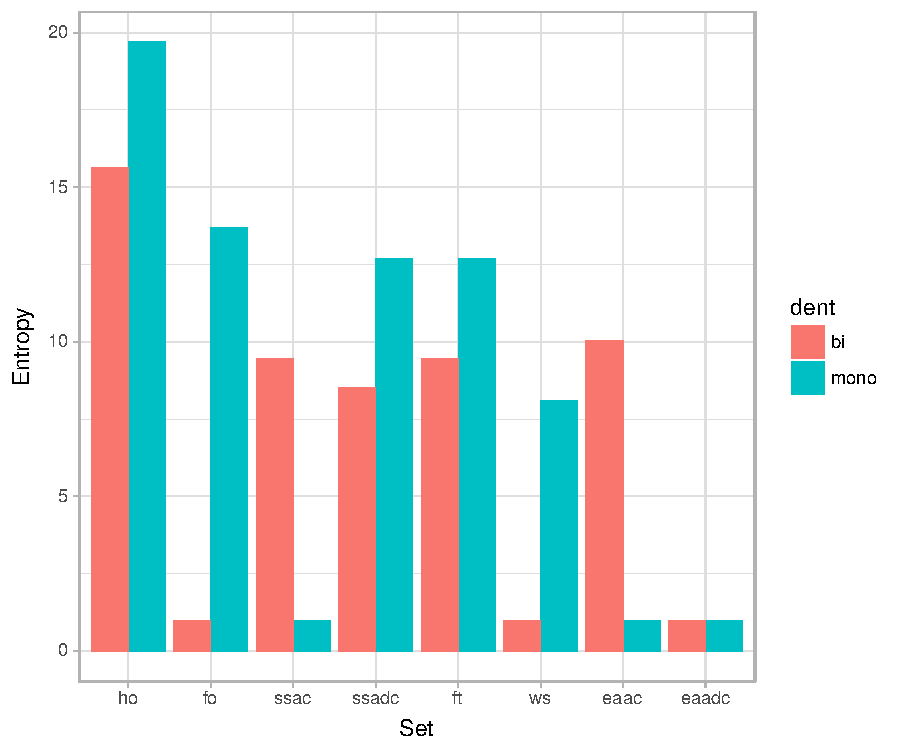
\includegraphics[width=0.7\linewidth]{img/ent.pdf}
%\end{figure}
%\end{frame}
%
%%
%%\begin{frame}
%%\frametitle{Actual calculations}
%%The calculations, colored by convergence fitness.
%%\begin{figure}
%%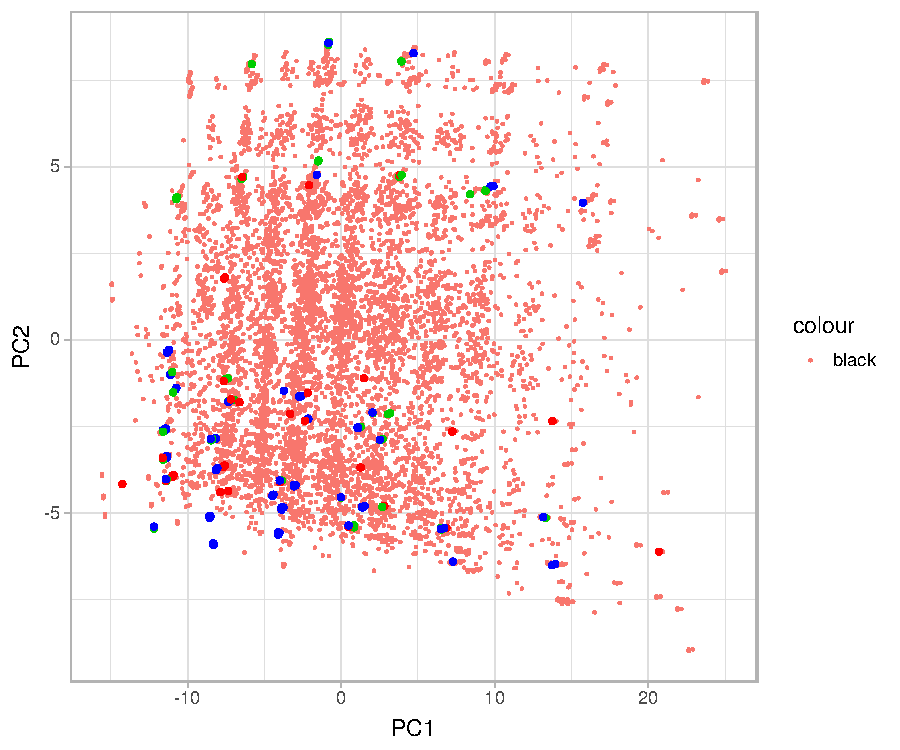
\includegraphics[width=0.7\linewidth]{img/pcaWithCalcs.pdf}
%%\end{figure}
%%\end{frame}
%
%\begin{frame}
%\frametitle{Actual calculations}
%\begin{figure}[ht] 
%	\label{ fig7} 
%	\begin{minipage}[b]{0.5\linewidth}
%		\centering
%		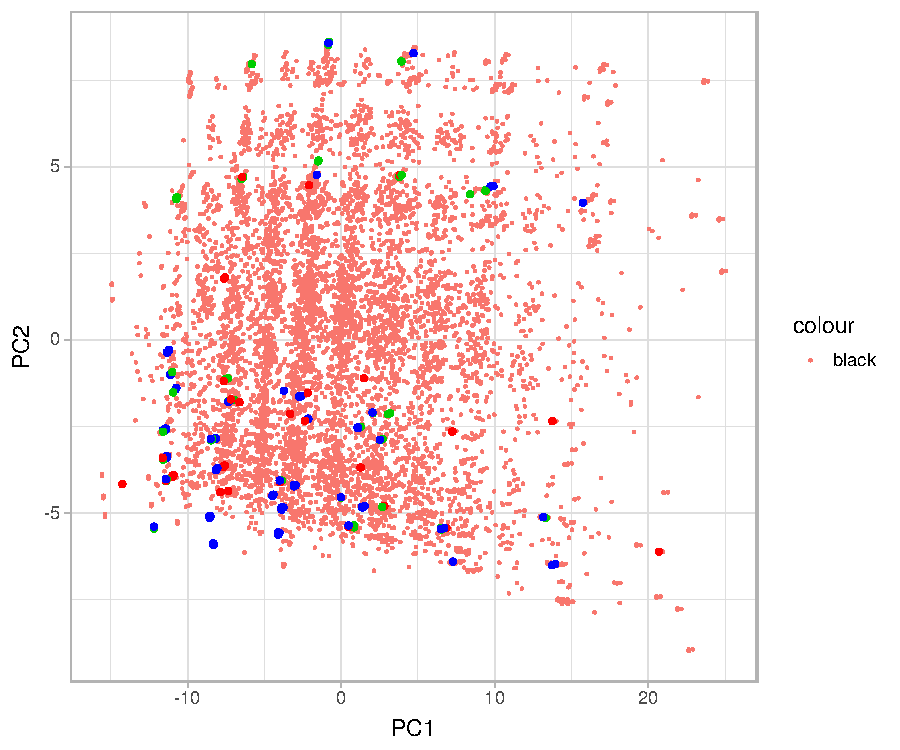
\includegraphics[width=.6\linewidth]{img/pcaWithCalcs.pdf} 
%%		\vspace{8ex}
%	\end{minipage}%%
%	\begin{minipage}[b]{0.5\linewidth}
%		\centering
%		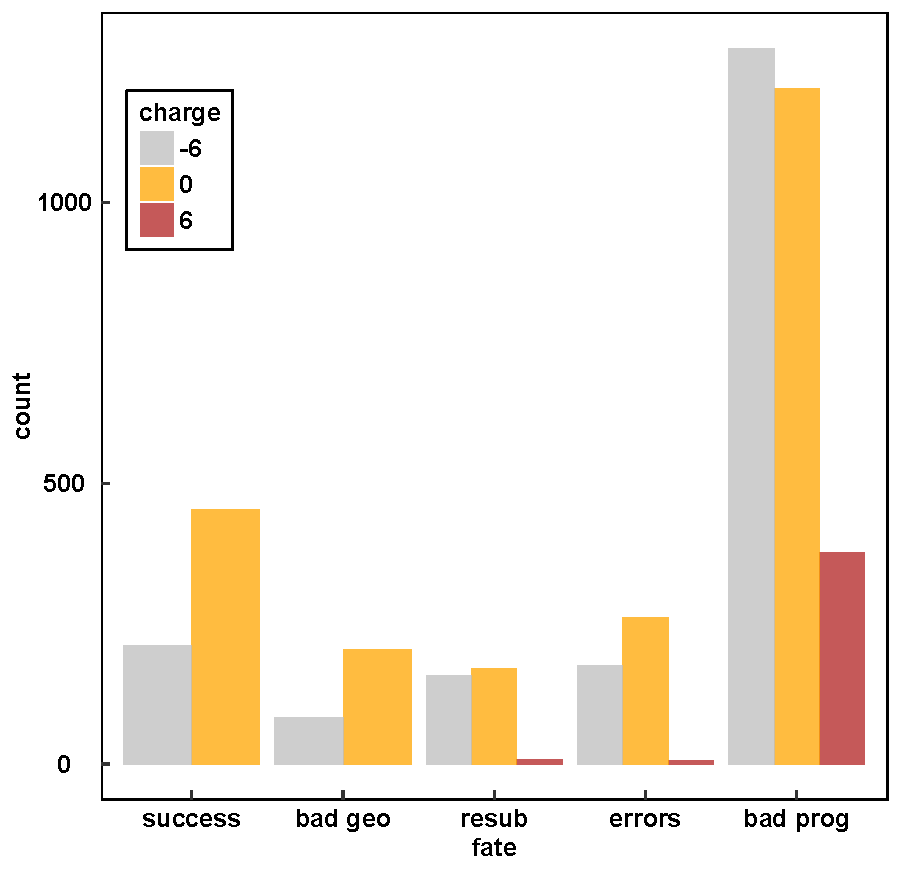
\includegraphics[width=.6\linewidth]{img/fateByCharge.pdf} 
%%		\vspace{8ex}
%	\end{minipage} 
%	\begin{minipage}[b]{0.5\linewidth}
%		\centering
%		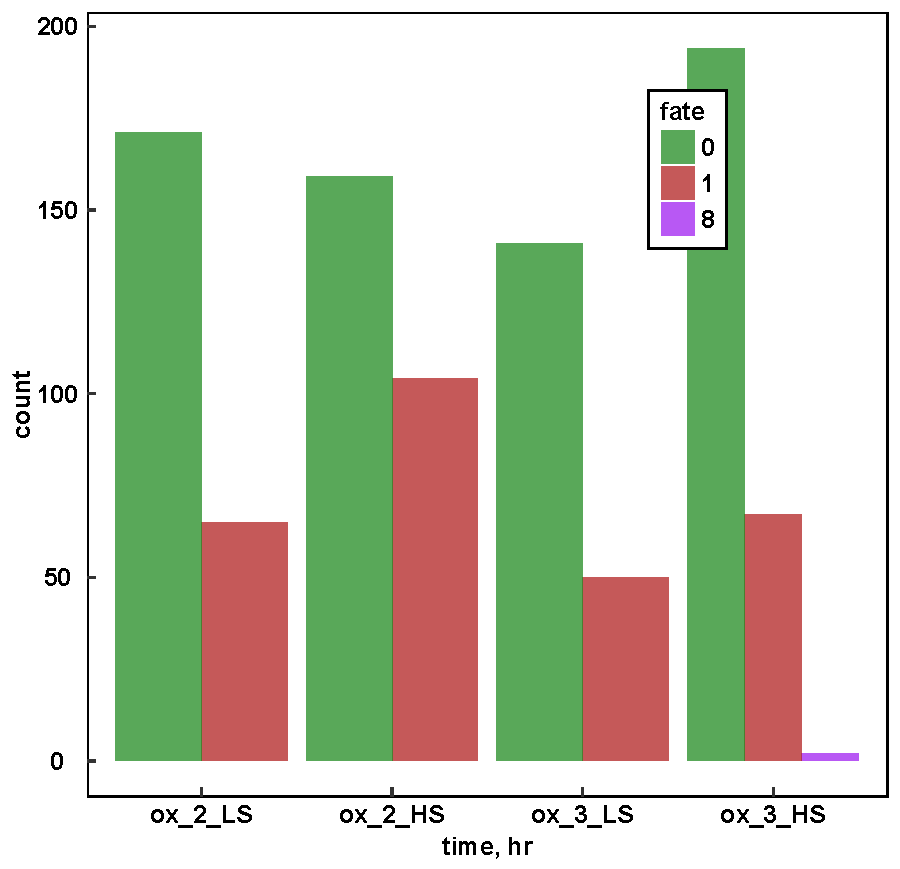
\includegraphics[width=.6\linewidth]{img/fateBytype.pdf} 
%%		\vspace{4ex}
%	\end{minipage}%% 
%	\begin{minipage}[b]{0.5\linewidth}
%		\centering
%		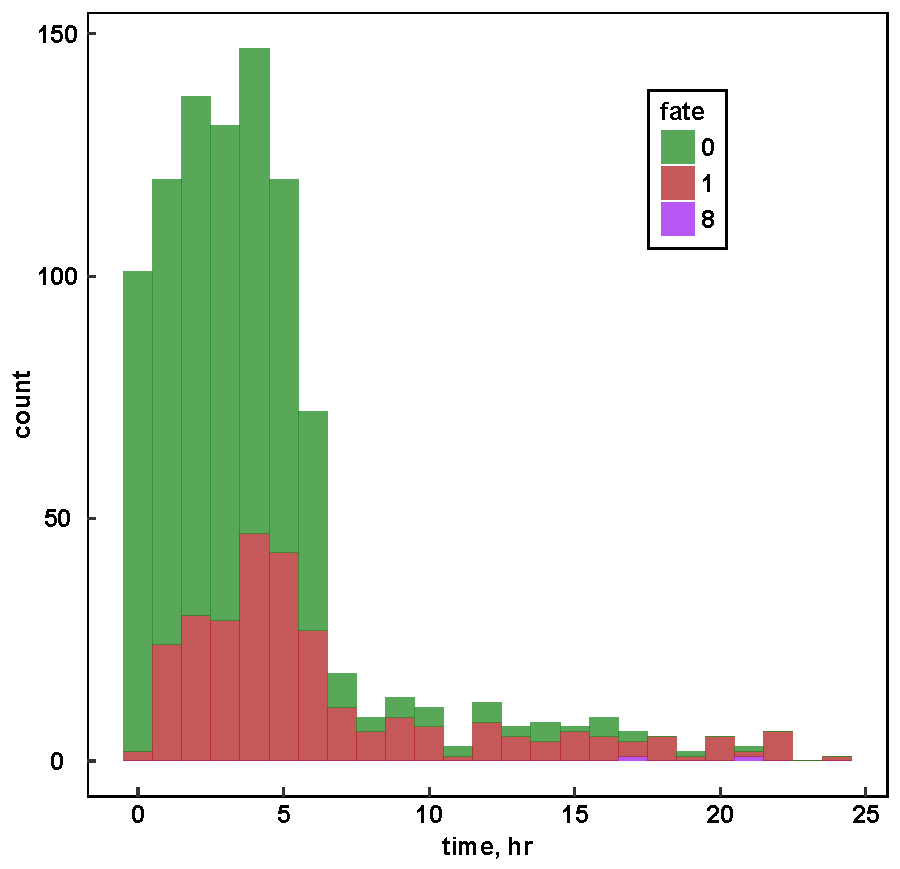
\includegraphics[width=.6\linewidth]{img/timeByfate.pdf} 
%%		\vspace{4ex}
%	\end{minipage} 
%\end{figure}
%\end{frame}
%
%
%\begin{frame}
%\begin{itemize}
%\item 0: [NH3], [N]\#[N], [C+]\#[O-], [C+]\#[NH-], [N]#[CH]
%\item 1: [CH+]=[CH3-], [NH]=[O], [CH+]=[OH-], [CH2+]-[OH2-]
%\item 8: [OH2-]-[PH+], [P+]=[OH-], [PH+]-[OH2-], [NH2-]=[CH+]
%
%\end{itemize}
%\end{frame}
